\documentclass{deliverablereport}

\usepackage[style=alphabetic,backend=bibtex]{biblatex}
\addbibresource{../../lib/kbibs/kwarcpubs.bib}
\addbibresource{../../lib/kbibs/extpubs.bib}
\addbibresource{../../lib/kbibs/kwarccrossrefs.bib}
\addbibresource{../../lib/kbibs/extcrossrefs.bib}
\addbibresource{../../lib/deliverables.bib}
%\addbibresource{../../lib/publications.bib}
\addbibresource{rest.bib}
% temporary fix due to http://tex.stackexchange.com/questions/311426/bibliography-error-use-of-blxbblverbaddi-doesnt-match-its-definition-ve
\makeatletter\def\blx@maxline{77}\makeatother

\usepackage{calbf}
\usepackage{wrapfig}
\usepackage{tikz}
\usetikzlibrary{positioning}
\usetikzlibrary{shapes.geometric}
\usetikzlibrary{shadows}
\usetikzlibrary{patterns}
\usetikzlibrary{arrows}
\usetikzlibrary{backgrounds}
\usetikzlibrary{mmt}
\usetikzlibrary{docicon}
\usetikzlibrary{tikzmark}
\usetikzlibrary{fit}
\usetikzlibrary{decorations,decorations.markings,decorations.text,decorations.pathmorphing}
\usepackage{standalone}
\usepackage[show]{ed}
\usepackage{listings}
\lstset{columns=fullflexible,basicstyle=\sf,language=Python}
% Variant: we could just provide the deliverable label as in the
% proposal, and fetch all the information from final.pdata
\usepackage{mdframed}
\newenvironment{boxedquote}
{\begin{mdframed}[leftmargin=1cm,rightmargin=1cm]}
{\end{mdframed}}
\deliverable{UI}{adcomp}
\deliverydate{02/27/2017}
\duedate{02/27/2017 (Month 18)}
\def\pn{OpenDreamKit}
\author{Michael Kohlhase \&  Tom Wiesing\\FAU Erlangen-N\"urnberg\\\url{http://kwarc.info} }

\begin{document}
\maketitle
%  Work Package WP6 develops a novel, foundational, knowledge-based framework for
  interfacing existing open source mathematical software systems and knowledge bases into
  a mathematical VRE, where systems can delegate functionalities among each other
  seamlessly without losing semantics.

  The overall Math-in-the-Middle (MitM) Framework developed in WP6 over the last three
  years is described in D6.5; this Report complements it by describing the curated
  contents Math-in-the-Middle (MitM) Ontology which serves as a reference and pivotal
  point for translations between the various input languages of mathematical software
  systems and knowledge bases.

  In a nutshell, the MitM Ontology describes the mathematical objects, concepts, and their
  relations in a general, system-agnostic way in an OMDoc/MMT theory graph while the
  mathematical systems export API theories that describe the system interface language in
  terms of types, classes, constructors, and functions -- again in OMDoc/MMT. These two
  levels of descriptions are linked by OMDoc/MMT alignments that allow the translation of
  expressions between systems.

%%% Local Variables:
%%% mode: visual-line
%%% fill-column: 5000
%%% mode: latex 
%%% TeX-master: "report"
%%% End:

\strut\githubissuedescription
\newpage\tableofcontents\newpage

\section{Introduction}\label{sec:intro}

\begin{newpart}{MK: adapted from Tom's Thesis}
There is a large and vibrant ecosystem of open-source mathematical software systems.
These systems can range from calculators, which are only capable of performing simple
computations, via mathematical databases (curating collections of a mathematical objects)
to powerful modeling tools and computer algebra systems (CAS). 

Most of these systems are very specific -- they focus on one or very few aspects of
mathematics.  For example, the ``Online Encyclopedia of Integer Sequences''
(OEIS~\cite{Sloane:oeis12,oeis}) focuses on sequences over $\mathbb{Z}$ an their
properties and the ``L-Functions and Modular Forms Database''
(LMFDB)~\cite{Cremona:LMFDB16,lmfdb:on} objects in number theory pertaining to Langland's
program.  GAP~\cite{GAP:on} excels at discrete algebra, whereas
SageMath~\cite{SageMath:on} focuses on Algebra and Geometry in general, and
Singular~\cite{singular:on} on polynomial computations, with special emphasis on
commutative and non-commutative algebra, algebraic geometry, and singularity theory.

For a mathematician however (a user; let us call her Jane) the systems themselves are not relevant, instead she only cares about being able to solve problems. 
Typically, it is not possible to solve a mathematical problem using only a single program. 
Thus Jane needs to work with multiple systems and combine the results to reach a solution. 
Currently there is very little help with this practice, so Jane has to isolate sub-problems the respective systems are amenable to, formulate them into the respective input language, collect results, and reformulate them for the next system a tedious and error-prone process at best, a significant impediment to scientific progress in its overall effect. 
Solutions for some situations certainly exist, which can help get Jane unstuck, but these are ad-hoc and for specific, often-used system combinations only. 
Each of these requires a lot of maintenance and does not scale to a larger set of specialist systems. 

The OpenDreamKit project, which aims at a mathematical VRE toolkit, proposes the Math-in-the-Middle (MitM~\cite{DehKohKon:iop16}) Paradigm, an interoperability framework based on a flexiformal
representation of mathematical knowledge and aligns this with system-generated interface
theories. 

In this paper we instantiate the MitM paradigm with a concrete domain development and
evaluate it on a distributed computing GAP, SageMath and Singular.\ednote{ we generally we
  want to show that the promises in the CICM paper become reality.}

We will use the following example as a running example: Jane wants to act on singular
polynomials with GAP permutation groups\ednote{MK@(MP|VA): }

 \ednote{MK: continue with the structure} 
\end{newpart}

%%% Local Variables:
%%% mode: latex
%%% TeX-master: "paper"
%%% End:
\newpage
\section{Examples of In-Situ Computation}\label{sec:examples}

In the following we will look at some examples to get a feeling for the applications.

\subsection{Unit Conversions}\label{sec:units}
Reading documents which contain units that one is not familiar with, can be an
annoying task, especially when uncommon units, such as solar masses or
fortnight, occur in the document or when a document is written in a system of
measurement different from the one the reader is used to.  A google query or a
similar service can automatically convert units, but this requires the reader
to leave his document. Instead, in-situ computation is a great
application for this purpose. In comparison to existing unit conversion web
services, this can also convert all expressions in a document --- without any
noticeable effort for the user. 


\subsection{Equations}\label{sec:equations}

A common example of in-situ computation is the exploration of mathematical models that are
given as equations. In the simplest case, this can be equations like Einstein's
mass-energy equivalence (\ref{f:emc2}) -- which we will use as a running example -- and in
other cases, this can be complex models like van Roosbroeck's models for drift and
diffusion of electrons and holes in semiconductor devices~\cite{FarRotDoa:nmddm16}\footnote{We
  are currently studying this model, formalizing the inherent knowledge and augmenting
  (parts of) \cite{FarRotDoa:nmddm16} into an active document, see~\cite{KohKopMueTab:RCS} for
  first results. The methods reported on here will eventually be employed in this case
  study, which itself is beyond the scope of this deliverable report}, which comprises
partial differential equations, boundary conditions, and physical constants -- a much more
complex situation, but the possible interactions are essentially the same. 

So let us come back to our running example: The equation for mass-energy equivalence is
simple:

\begin{equation}\label{f:emc2}
  E=mc^2
\end{equation}

where $E$ is the energy, $m$ is the mass, and $c$ is the speed of light. It appears in
many documents, e.g. the Wikipedia article in Figure~\ref{fig:emc2-wikipedia}. In such a
document -- were it active -- a scholar or interested layman might be interested to see
what the energy equivalent of one gram of matter might be. Today a google query reveals a
custom-made answer at~\cite{Odenwald:q388}, but really our scholar would like to just right
click on the symbol $m$ in $\ref{f:emc2}$, instantiate it to $1g$ and have the document
\emph{simplify the changed expression} (in-situ computation) to give the answer.

Conversely, she might want to know how what mass it would take to drive e.g. from Erlangen
to Paris in a Tesla (which gets 6.25 km per kWh)\footnote{This is a natural and common
  question; see~\cite{RT:emc2} which computes the mileage a car would get out of a 1/16
  inch drop of water -- the value it comes up with is 96.000 miles.}. Here she would like
to just instantiate $E$ with $776 \times 6.25=4850$ kWh and the document \emph{solves the
  equation $4850=mc^2$ for $m$}.\ednote{MK: maybe do the computation and report the
  result} Of course, the result is so minuscule that she wants to have it changed to a
form she understand, e.g. the number of carbon atoms that weigh as much.

\begin{figure}\centering
  \begin{boxedquote}
    In physics, mass–energy equivalence states that anything having mass has an equivalent
    amount of energy and vice versa, with these fundamental quantities directly relating
    to one another by Albert Einstein's famous formula:

    \[E=mc^2\] 

    This formula states that the equivalent energy ($E$) can be calculated as the mass ($m$)
    multiplied by the speed of light ($c$ = about $3\times10^8 m/s$) squared.
  \end{boxedquote}
  \caption{From the Mass-Energy-Equivalence page at Wikipedia~\cite{WP:emc2}}
  \label{fig:emc2-wikipedia}
\end{figure}

Of course, the computations themselves in our example are rather simple, and can be
executed by any computer algebra system, and even complex examples like the van Roosbroeck
models alluded to above would tax modern systems exceedingly, indeed they are the kind
computations that are carried out and documented in Jupyter notebooks. 

The point here is that the envisioned in-situ computation service allows computation
without changing to another system and avoids errors (data entry errors and data
interpretation errors) induced by crossing system borders.

\subsection{Computation with Proofs}
\begin{itemize}
  \item calling automated theorem provers on a goal in a document
  \item extending the level of explanation by doing that on a subgoal or deepening the
    level of explanation. E.g. from ``obviously'' to a full proof.  
  \end{itemize}

\subsection{Hypothetical Computations Playing with Global/Local Values}\label{sec:hyp}
What would be paper look like if the speed of light were $88 mph$. 

\subsection{Updating Values to current or historical values}
spreadsheets (a well-understood form of active documents) can already do that. 
\begin{itemize}
\item global warming papers with newer models or data
\item Wolfram alpha: ``does it snow in hell?''
\end{itemize}




%%% Local Variables:
%%% mode: latex
%%% TeX-master: "report"
%%% End:

%  LocalWords:  sec:examples sec:units sec:equations f:emc2 Roosbroeck's Kopruckietal
%  LocalWords:  formalizing KohKopMueTab:RCS fig:emc2-wikipedia Odenwald:q388 emph
%  LocalWords:  RT:emc2 centering boxedquote WP:emc2 Roosbroeck Jupyter itemize sec:hyp
\newpage
\section{Information Architecture}\label{sec:infarch}

\begin{oldpart}{some intro here}
  Documents have Math Objects (encoded in content and presentation MathML)\ednote{the
    former may be in the content commons in the Active Documents Figure} and the documents
  have a context \ednote{The guy from Eindhoven had something about document and user
    context here.~\cite{Verrijzer:cimdpm15} in the context of the MathDox
    system~\cite{mathdox:on}} that explains/binds all symbols in the object. This context
  must be some how represented in the document and has to be transmitted to the
  computation service.
\end{oldpart}

To get a feeling for the situation, consider Figure~\ref{fig:emc-adp} which instantiates
the abstract diagram from Figure~\ref{fig:activedocs} to the situation in our running
example: Einstein's energy/mass equivalence. We have the two parts: the document commons
with (a slightly rephrased fragment of) the document in Figure~\ref{fig:emc2-wikipedia}
on the left upper corner and the content comment on the other side of the dashed line. 

The latter is encoded as an OMDoc/MMT theory graph -- see~\cite{RabKoh:WSMSML13} for
technical details and~\cite{DehKohKon:iop16,ODK-D6.2} for an account of the applications
in the \pn project. All relevant concepts are grouped in named theories (the boxes with
rounded corners), which introduce symbols and their properties e.g. the definition of the
unit Joule in \textsf{energy} or the size of the speed of light in
\textsf{lightspeed}. These theories are connected by theory morphisms -- only inclusions
$S\mmtar{include}T$ which make all declarations (symbols and properties) of $S$ visible in
$T$ -- and give an object-oriented, modular regime of formalizing mathematical knowledte.

\begin{figure}\centering
  {\footnotesize\documentclass{standalone}
\usepackage{amsfonts}
\usepackage{tikz}
\usetikzlibrary{tikzmark}
\usetikzlibrary{mmt}
\usetikzlibrary{docicon}
\begin{document}
\def\cn#1{\mathsf{#1}}
\def\bT{\mathbb{T}}
\def\bL{\mathbb{L}}
\def\bM{\mathbb{M}}
\def\bE{\mathbb{E}}
\begin{tikzpicture}[xscale=2,yscale=2,remember picture]
  \tikzstyle{doc}=[draw,color=black,shape=document]

  \node[thy] (m) at (0,0) {$\mmtthy{mass}{\subnode{cma}{\ensuremath\bM}:\cn{type},g:\bM,kg:\bM,\ldots}{}$}; 
  \node[thy] (l) at (2,0) {$\mmtthy{length}{\bL:\cn{type},m:\bL,\ldots}{}$};
  \node[thy] (t) at (4,0) {$\mmtthy{time}{\bT:\cn{type}, s:\bT,h:\bT,\ldots}{}$}; 
  \node[thy] (e) at (2,1) {$\mmtthy{energy}{\subnode{cen}{\ensuremath\bE}:\cn{type},J:\bE,\ldots}{1J=1\frac{kg\cdot m^2}{s^2}}$};
  \node[thy] (c) at (4,1) {$\mmtthy{lightspeed}{\subnode{clv}{\ensuremath{c}}:\bL/\bT}{1c= 299 792 458\frac{m}{s^2}}$}; 
  \node[thy] (emc2) at (4,2) {$\mmtthy{EME}{E:\bE,m:\bM}{E=mc^2}$}; 
  \draw[include] (t) -- (e);
  \draw[include] (l) -- (e);
  \draw[include] (m) -- (e);
  \draw[include] (t) -- (c); 
  \draw[include] (l) -- (c); 
  \draw[include] (c) -- (emc2); 
  \draw[include] (e) -- (emc2); 

  \node[doc,thick] (snip) at (-.3,1.8) 
  {\begin{minipage}{3.8cm}
      \[E=mc^2\] where \fbox{$E$ is the \subnode{den}{Energy}}, \fbox{$m$ is the \subnode{dma}{Mass}}, and
      \fbox{\subnode{cls}{$c$} the \subnode{dlv}{speed of light}}.
    \end{minipage}};
  \draw[dashed,->] (den) -- (cen);
  \draw[dashed,->] (dma) -- (cma); 
  \draw[dashed,->] (dlv) to[bend left=25] (clv); 
\end{tikzpicture}
\end{document}

%%% Local Variables:
%%% mode: latex
%%% TeX-master: t
%%% End:
}
  \caption{$E=mc^2$ as an Active Document}\label{fig:emc-adp}
\end{figure}

Documents are marked up in terms of its document, statement, and phrase structure in the
ADP. In particular, we mark up
\begin{enumerate}
\item the sectioning structure -- omitted in our running example, 
\item statements -- the assertion for $E=mc^2$ coincides with the whole document
  \dociconprototype{D} in Figure~\ref{fig:emc-adp}, and
\item the phrase structure -- here declarations are shown as boxes and technical terms as
  dashed boxes.
\end{enumerate}
Finally, the marked up structures in the document commons are cross linked to the content
commons to create \textbf{parallel markup}\footnote{The idea of ``parallel markup'' has
  been pioneered by the MathML format~\cite{CarlisleEd:MathML3:base}, which uses it to
  connect equivalent sub-formulae in presentation and content Markup, and~\cite{Iancu:phd}
  generalizes it to all levels in the OMDoc/MMT setting.} at all levels. We see three
dashed arrows: two connect the technical terms ``Energy'' and ``Mass'' in the dashed boxes
to the corresponding concepts in the content tree and one that connects the whole
declaration ``$c$ is the speed of light'' to the corresponding declaration in the theory
\textsf{ligthspeed}. The dotted arrow on the top of Figure~\ref{fig:emc-adp} represents
still another parallel alignment relation, it is the ``home theory'' relation, which makes
all concepts from a theory -- the \textbf{home theory}; here \textsf{EME} -- in a document
fragment. All parallel markup relations must be refinements of this relation to be
well-justified in OMDoc/MMT.

The crucial observation is that together, the home theory relation, its refinements, and
the document markup give a notion of context for the computation. The (required)
declarations for the local identifiers $E$ and $m$ in \dociconprototype{D}, and the
(optional) declaration for the identifier $c$ inherited form the theory
\textsf{lightspeed} give meaning to $E=mc^2$ and also determine what can be
computed. Instantiating the \emph{variables} (locally declared identifiers) $m$ and $E$
give rise to the computations in Section~\ref{sec:equations}, whereas the ``replacing''
the \emph{constant} (an identifier inherited from a theory) $c$ with a different value the
hypothetical calculations from section~\ref{sec:hyp}. We can even predict the grade of
hypotheticality by the inheritance distance in the content theory graph.

Formally, the \textbf{computation context} of a formula comes in the form of
\textbf{declarations}, i.e. triples of the form $c:\tau=\delta$, where $c$ is the name of
the declared identifier, (optionally) $\tau$ its type $\tau$, and (again optionally) a
definiens $\delta$. In our running example, the context of $E=mc^2$ consists of three
declarations: $E:\bbE$, $m:\bbM$, and $c:\bbL/\bbT=299 792 458$ (leaving out units for the
moment). It can be inferred from the information in Figure~\ref{fig:emc-adp}; but let us
make the active document fragment more explicit. 

Listing~\ref{lst:emc-adfragment}\ednote{MK: I am sure that MMT generates something
  slightly similar, update when we know} shows the HTML5 representation for the active
document fragment in Figure~\ref{fig:emc-adp}. It shows the (presentation) MathML
representation of $E=mc^2$, followed by the text part in which the declarations are marked
up with \lstinline|span| elements of class \lstinline|o_declaration| for the variable
declarations and \lstinline|o_symbol| for the symbol declaration. These carry the
OMDoc/MMT attributes \lstinline|o:for| and \lstinline|o:scope|. The former points to the
identifier being declared, and the latter points at the element in which this declaration
is active. In this case, since the scope is the other \lstinline|<p>| element the
declarations govern the identifiers in the displayed equation $E=mc^2$. 

\begin{lstlisting}[label=lst:emc-adfragment,caption=Native Markup for an Active Document Fragment, 
language=HTML,basicstyle=\footnotesize\sf,mathescape,morekeywords={mi,mo,msup,math,mrow}]
<p id="p" xmlns:o="http://omdoc.org/ns">
 <math display="block" xref="http://mathhub.info/phys/famous?equations?eme">
  <mi>E</mi>
  <mo>=</mo>
  <mrow>
   <mi>m</mi>
   <mo>&invisibletimes;</mo>
   <msup><mi>c</mi><mn>2</mn></msup>
  </mrow>
 <math>
 where 
 <span class="o_declaration" o:for="#E" o:scope="#p">
  <math><mi id="E">E</mi></math> is the 
  <span class="term" xref="http://mathhub.info/units/SI/complex?energy?$\bbE$">energy</span>
 </span>,
 <span class="o_declaration" o:for="#m" o:scope="#p">
  <math><mi id="m">m</mi></math> is the 
  <span class="term" xref="http://mathhub.info/units/SI/dimensions?mass?$\bbM$">mass</span>
 </span>, and 
 <span class="o_symbol" o:for="#c" o:scope="#p">
  <math><mi id="c" xref="http://mathhub.info/phys/const/basic?lightspeed?c">c</mi></math> the 
  <span class="term" xref="http://mathhub.info/phys/const/basic?lightspeed?lightspeed">speed of light</span>
 </span>.
</p>
\end{lstlisting}

\begin{wrapfigure}r{7cm}\vspace*{-.5em}
\begin{lstlisting}[language=XML,morekeywords={constant,type,apply,math,ci,cn,csymbol},basicstyle=\footnotesize\sf]
<constant name="eme">
 <type>
  <math>
   <apply><eq/>
    <ci>E</ci>
    <apply><times/>
     <ci>m</ci>
     <apply><power/>
      <csymbol cd="lightspeed">c</ci>
      <cn>2</cn>
     </apply>
    </apply>
   </apply>
  </math>     
 </type>
</constant>
\end{lstlisting}
  \caption{$E=mc^2$ in Content MathML}\label{fig:emc-content}
\end{wrapfigure}
Now let us have a look at how this enables computation: The displayed equation $E=mc^2$
linked into the content commons via its \lstinline|xref| attribute, which points to the
(constant) declaration in Figure~\ref{fig:emc-content}. The \lstinline|constant| element
combines the system name \lstinline|eme| with the statement of the equation in the
\lstinline|type| element\footnote{This is a consequence of using the Curry/Howard
  isomorphism at work; we have elided the details of the type here.}. As the equation is
represented as the ``operator tree'' in content MathML, it is fully disambiguated
functionally and can therefore directly be computed with in a computational engine
(e.g. the MMT system itself or a computer algebra system like GAP or SageMath) after
instantiation of the variables with concrete values.


\subsection{Information Architecture for Unit Conversion}
For the automatic conversion of units, we assume that the document contains formulas
in MathML with cross references between its presentational part and its content MathML. 
The content MathML needs to be annotated with the semantics of the expression, which
includes the information about the present units. 


%%% Local Variables:
%%% mode: latex
%%% TeX-master: "report"
%%% End:

%  LocalWords:  sec:infarch oldpart Verrijzer:cimdpm15 mathdox:on fig:emc-adp textsf emph
%  LocalWords:  fig:activedocs fig:emc2-wikipedia RabKoh:WSMSML13 mmtar formalizing mrow
%  LocalWords:  DehKohKon:iop16,ODK-D6.2 centering emc-adp dociconprototype textbf msup
%  LocalWords:  Iancu:phd ligthspeed sec:equations sec:hyp hypotheticality lstlisting
%  LocalWords:  sf,mathescape,morekeywords mi,mo,msup,math,mrow invisibletimes msup o:for
%  LocalWords:  xref lst:emc-adfragment lstinline lstinline lst:emc-adfragment,caption
%  LocalWords:  xmlns:o wrapfigure vspace constant,type,apply,math,ci,csymbol csymbol
%  LocalWords:  csymbol fig:emc-content
\newpage
\section{Implementation}\label{sec:impl}
The implementation of in-situ computation is organized along the information model outlined in
the last section.
It is realized as a set of Javascript modules in the JOBAD framework~\cite{JOBAD:on}, a Javascript framework for instrumenting (active) documents with user interactions; see~\cite{GLR:WebSvcActMathDoc09} for details.

We will first discuss unit conversion (see Section~\ref{sec:ex:units}) as a special case of in-situ computation and then generalize to the case of a non-trivial context and generalize to arbitrary computations in Section~\ref{sec:impl:general}.

\subsection{Unit Conversion}\label{sec:impl:units}
Unit conversion is a special case of in-situ computation, because
\begin{compactitem}
\item the computations are essentially limited to unit conversion and
\item context is trivial, since the computational objects -- the quantity expressions -- consist only of a number and a unit expression. The units are all defined constants and local identifiers do not exist.
\end{compactitem}
Ulrich Rabenstein of the KWARC group has implemented a semantics extraction procedure that finds quantity expression in HTML5 documents, analyzes their content structure and represents them in content MathML and stored as (standoff) RDF annotations.
These can be used to feed in-situ computations.

The user interface for unit conversion can be implemented directly in JOBAD by delegating the conversion (the content MathML representation of the quantity expressions has sufficient information) to a unit converter -- we use the units package from Astropy~\cite{astropy}, an extendible python library for astronomy -- whose result can be converted to Presentation MathML for inclusion in the document.
We show the user interaction here.

Before starting to convert something, the user can highlight all quantity expressions in a given document.
This results in a document, as shown in Figure~\ref{fig:highlight}.
We further use this snippet as an example.

\begin{figure}[ht]
    \fbox{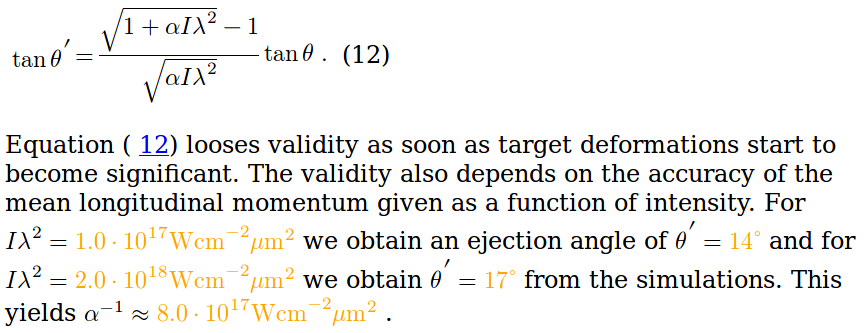
\includegraphics[width=\textwidth]{screenshots/highlight}}
    \caption{Highlighting Quantity Expressions in \cite{physics/9807021}}\label{fig:highlight}
\end{figure}

In the first case, the user wants to convert a unit in just one expression to an equivalent one, say watt to horsepower.
For that, she can right-click on this particular expression and choose a target unit (e.g.  horsepower) from the list of units that are equivalent to Watt.
Figure~\ref{fig:convertone} demonstrates this and Figure~\ref{fig:convertoneresult} displays the result of the computation.

\begin{figure}
  \begin{subfigure}{\textwidth}
    \fbox{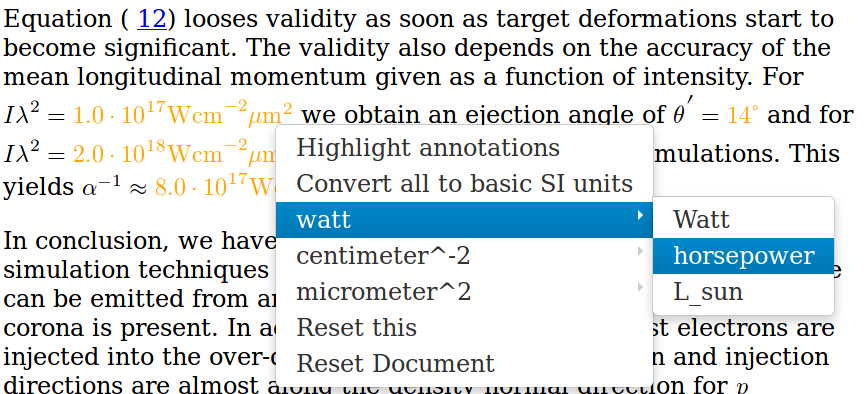
\includegraphics[width=\textwidth]{screenshots/convertone}}
    \caption{Choosing A Target Unit}\label{fig:convertone}
    \fbox{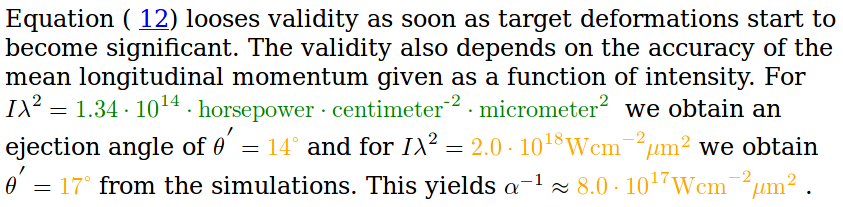
\includegraphics[width=\textwidth]{screenshots/convertoneresult}}
    \caption{The Result of converting one QE}\label{fig:convertoneresult}
    \fbox{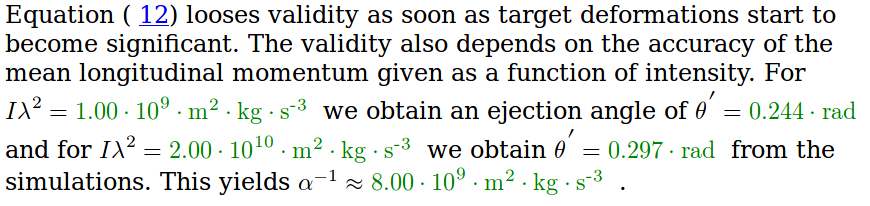
\includegraphics[width=\textwidth]{screenshots/si}}
    \caption{Converting a Document To SI}\label{fig:si}
  \end{subfigure}
  \caption{In-Situ Unit Conversion}\label{fig:unit-conversion}
\end{figure}

The current example only allows local conversions, but of course the user also wants to convert units document-wide -- ideally from one system of measurement to another.
Figure~\ref{fig:si} shows the result of a prototypical implementation, which converts all units to irreducible SI base units.
This could, for instance, be extended to automatically convert all quantity expressions in a document from imperial to metric units and vice versa.

\subsection{A General Framework for In-Situ Computation}\label{sec:impl:general}

In addition to the example above, we have also implemented a prototype of the general in-situ computation manager detailed above.
A right click on a formula $F$ triggers the JOBAD menu, which has an ``Active Computation'' field.

  \begin{itemize}
  \item First, the \textbf{context extractor}, a function that for all the \lstinline|ci| elements in the content formula $C$ associated with $F$, and tries to find the associated variable declarations by going up the parent chain of $F$ and the symbol declarations from the home theory.
  Note that using the content MathML representation $C$ of $F$ gets us around disambiguation problems: even if the presentation of $F$ is ambiguous (e.g. by using variable or constant names multiple times), $C$ is not.
  \item The variable context is displayed to the user prompting instantiation in a popup form: the \textbf{in-situ computation manager} (see Figure~\ref{fig:compman}, which allows to give values for the components of the equation, pick different actions (simplification, equation solving, \ldots ) and ways of providing the results (in-place, footnote, \ldots ).
  As the current system is only a prototype, one can currently only select the Evalutation Action.
  \item In a second step, the  user-supplied values are parsed into content MathML, inserted into $C$, yielding the content MathML expression $C'$, which is then shipped to the computational engine.
  Currently we only support the MMT system as a computational engine, but this is not a restriction, since MMT can delegate computations to engines like GAP, Sage, PARI, \ldots via the SCSCP protocol~\cite{ODK-D3.3}.
  \item Finally, the result $R$ of computing $C'$ -- a content MathML expression -- is inserted back into the original computation context.
  This context can then be presented in presentation MathML and inserted into the document according to the method the user selected \footnote{
  Currently, the system presents the user with the computed context directly. }.
  \end{itemize}

  \begin{figure}[ht]\centering
    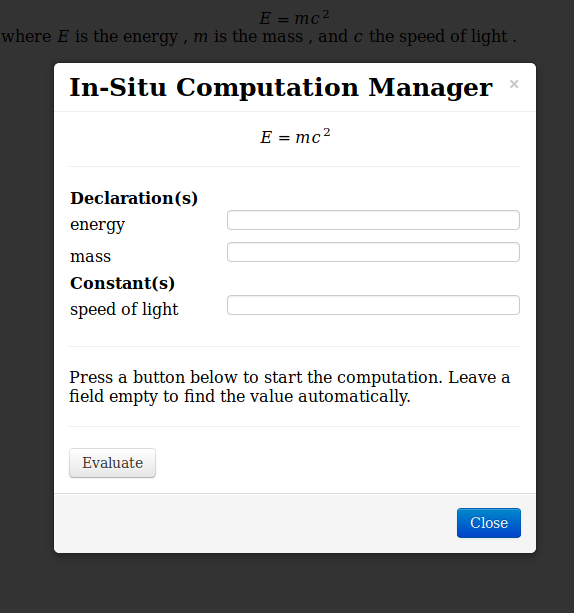
\includegraphics[width=12cm]{screenshots/compman}
    \caption{In-Situ Computation Manager}\label{fig:compman}
  \end{figure}

\subsection{Code Availability, Licensing and Demos}

For both of the examples in this section, an implementation is available under Open Source license terms.
For reasons of lacking MathML support in other browsers, we have only tested these demos in Firefox.

A demo of the unit conversion is available at \url{http://ash.eecs.jacobs-university.de/}.
A user can first select a document and then repeat the procedure detailed above in Section~\ref{sec:impl:units}.
The source code of the demo is available in the repository at \url{https://gl.kwarc.info/urabenstein/Semanticextraction/tree/master/server}.
The server can be executed locally following the steps in the corressponding README file.

A protoype of the General Framework for In-Situ Computation is also availble.
It can be found at \url{http://ash.eecs.jacobs-university.de/prototype/} and shows the basics of the process explained in Section~\ref{sec:impl:general}.
it consists of a frontend component, the source code of which can be found at \url{https://gl.mathhub.info/ODK/ActiveComputationDemo}, as well as a backend component inside the MMT system.
The source code to the backend component can be found at \url{https://github.com/UniFormal/MMT/tree/master/src/mmt-odk/src/info/kwarc/mmt/odk/activecomp}.

%%% Local Variables:
%%% mode: latex
%%% TeX-master: "report"
%%% End:
\newpage
\section{Conclusion}\label{sec:concl}
We have surveyed the two document-formed user interfaces in the \pn project: Jupyter
Notebooks and Active Documents and developed a joint perspective on them that allows us to
propose a joint generalization oft the functionalities combines their respetive
advantages. We feel that embedding computations in arbitrary places in traditional
mathematical documents forms a natural generalization of the two existing user
interfaces. In particular the appearance as ``enhanced mathematical documents'' may make
the VRE more natural to mathematicians who have little experience with symbolic
computation tools, as they naturally have experiences with paper articles and textbooks
from their studies.

The survey and outlook provided by this report will be used as a basis for the discussion
of an integrated user interface and in the \pn project (WP4). As integration of knowledge
and computation (and interoperability between the various system involved) is a central
theme of WP6, this will require interaction between the work packages.

\subsection*{Acknowledgements} The authors are grateful to Min RK from Simula for
discussions on the inner workings of Jupyter and help with initial experiments with
setting up a a MMT kernel for Jupyter. Florian Rabe, Dan Alistarh, and Tom Wiesing have
worked on an initial integration of MMT with Jupyter that shaped and validated the vision
for an integrated user interface for the \pn VRE formulated in this report. Discussions
with Nicolas Thierry have refined the ideas presented here.

%%% Local Variables:
%%% mode: latex
%%% TeX-master: "report"
%%% End:
\newpage
\printbibliography
\end{document}

%%% Local Variables:
%%% mode: latex
%%% TeX-master: t
%%% End:

%  LocalWords:  githubissuedescription newpage tableofcontents newpage printbibliography
%  LocalWords:  maketitle
